\pdfpagewidth=8.5in
\pdfpageheight=11in

\documentclass{sig-alternate}
\usepackage[utf8]{inputenc}
\usepackage[T1]{fontenc}
\usepackage{microtype}

\usepackage{url}
\usepackage{amsmath}
\usepackage{graphicx}
\usepackage{subfigure}
\usepackage{threeparttable}
\usepackage{pdflscape}
\usepackage{array}
\usepackage{color}

\usepackage{flushend}

\clubpenalty = 10000
\widowpenalty = 10000
\displaywidowpenalty = 10000

\begin{document}

\conferenceinfo{MSR}{'15, May 16 – 17, 2015, Florence, Italy}
\CopyrightYear{2015}
\crdata{978-1-4503-2863-0/14/05}

\title{The Three Corridors}

\numberofauthors{5}

\def\aueb{\textsuperscript{*}}
\def\tud{\textsuperscript{\dag}}

\author{
  Vassilios Karakoidas\aueb \and Dimitris Mitropoulos\aueb \and Panos Louridas\aueb \and Georgios Gousios\tud \and Diomidis Spinellis\aueb \\
  \begin{tabular}{ccc}
  \affaddr{\aueb Department of Management Science and Technology} & & \affaddr{\tud Software Engineering Research Group}\\
    \affaddr{\aueb Athens University of Economics and Business} & & \affaddr{\tud Delft University of Technology}\\
   \affaddr{Athens, Greece} & & \affaddr{Delft, the Netherlands}\\
   \email{\{bkarak,dimitro,louridas,dds\}@aueb.gr}& & \email{g.gousios@tudelft.nl} \\
  \end{tabular}
}

\maketitle
\begin{abstract}

\end{abstract}

\category{D.2.4}{Software Engineering}{Software/Program Verification}[Statistical methods]
\category{D.2.7}{Software Engineering}{Distribution, Maintenance, and Enhancement}[Version control]

\terms{Static Analysis, Software Ecosystems.}

\keywords{Maven Repository, JDepend, Software Metrics, Chidamber and Kemerer.}


\section{Introduction}
\label{sec:intro}

Software metrics provide a means to extract useful and measurable information about the structure of a software system. Since software artefacts consist of digital data, many of their aspects are easily measured. This explains why the first metrics like LOC (Lines Of Code) and CLOC (Comment Lines of Code) appeared very early. Over the years, a wealth of different metrics has appeared in the literature \cite{GUSC07,BBM96,LOKI94,HK81,BDM97} and some of them, like Chidamber and Kemerer \cite{CHKE94} have found their way in software development practice and tools.

Today a software engineer or developer has a very large list of metrics at his disposition in order to gain the required insight for understanding and evaluating the size, complexity and overall structure of a system.

\section{Dataset Contents}
\label{sec:data}

 Maven is a build automation tool used primarily for Java projects, and it is hosted by the Apache Software Foundation\footnote{\url{http://www.apache.org/}}. To describe the software project being built, its dependencies on other libraries, and the build order Maven uses {\sc xml}. The repository contains more than 400,000 {\sc jar}s, in a variety of languages that are all using the {\sc jvm} platform as basis. These languages include Java, Clojure, Groovy, and Scala.

Initially, a snapshot (January 2012) of the Maven repository was downloaded locally. The repository contains various projects and their releases. A project version can be uniquely identified by the following triplet: {\it group id}, {\it artifact id} and {\it version}. The Maven repository contains several versions of each project.

All versions were filtered out and only the latest was kept. For each version in the Maven repository, each binary {\sc jar} file is accompanied by another {\sc jar}, which contains the source code. Table \ref{tbl:oss-size-metrics} presents several size metrics regarding the final version corpus. It included 12,959 projects, with more than 110 million lines of code.

\begin{itemize}
  \item \textbf{CKJM-ext} \textit{(ckjm)}\footnote{\url{http://www.spinellis.gr/sw/ckjm/}} is an open source tool that was developed by Diomidis Spinellis and then extended by Marian Jureczko. It calculates many software complexity metrics, including the \textit{Chidamber and Kemmerer} set of metrics \cite{CHKE94}.

  \item \textbf{JDepend} \textit{(jdep)}

  \item \textbf{CLMT} \textit{(clmt)}
\end{itemize}

\begin{table}
\centering
\caption{The selected Maven projects' size metrics}
\label{tbl:oss-size-metrics}
\begin{tabular}{l r}
 \hline
\textbf{Metric} & \textbf{Value}\\
\hline
Project Count & 12,959\\
File Count & 604,821\\
Module Count & 72,302\\
Lines of Code & 110,156,703\\
Source Lines of Code & 61,246,807\\
Comment Lines of Code & 36,696,217\\
Number of Classes & 499,588\\
Number of Interfaces & 89,145\\
Number of Enumerations & 12,732\\
\hline
\end{tabular}
\end{table}

\begin{table}
\centering
\caption{Key Metrics}
\label{tbl:selected-metrics}
\begin{tabular}{l l}
 \hline
\multicolumn{2}{l}{\textit{\textbf{Class Design}}}\\
\hline
Depth Of Inheritance Tree & \textit{ckjm}\\
Coupling Between Objects & \textit{ckjm}\\
Weighted Methods Per Class & \textit{ckjm}\\
Response For Class & \textit{ckjm}\\
Lack Of Cohesion In Methods & \textit{ckjm}\\
Number Of Children & \textit{ckjm}\\
Attribute Hiding Factor & \textit{clmt}\\
Coupling Between Methods & \textit{ckjm}\\
Average Method Complexity & \textit{ckjm}\\
Cohesion Among Methods of Class & \textit{ckjm}\\
Data Access Metric & \textit{ckjm, clmt}\\
Inheritance Coupling & \textit{ckjm}\\
Lack Of Cohesion In Methods3 & \textit{ckjm}\\
Measure Of Aggregation & \textit{ckjm}\\
Measure Of Functional Abstraction & \textit{ckjm}\\
Number of Attributes & \textit{clmt}\\
Method Hiding Factor & \textit{clmt}\\
\hline
\multicolumn{2}{l}{\textit{\textbf{Method Design}}}\\
\hline
Number of Method Parameters & \textit{clmt}\\
Number of Methods & \textit{clmt, ckjm}\\
McCabe Cyclomatic Complexity & \textit{ckjm, clmt}\\
\hline
\multicolumn{2}{l}{\textit{\textbf{Package Design}}}\\
\hline
Number of Concrete Classes & \textit{jdep}\\
Afferent Couplings & \textit{jdep, ckjm}\\
Efferent Couplings & \textit{jdep, ckjm}\\
Instability & \textit{jdep}\\
Abstractness & \textit{jdep}\\
Distance Main Sequence & \textit{jdep}\\
\hline
\multicolumn{2}{l}{\textit{\textbf{Program Size Metrics}}}\\
\hline
Number of Classes & \textit{clmt, ckjm, jdep}\\
Number of Enumerations & \textit{clmt, ckjm}\\
Number of Interfaces & \textit{clmt, ckjm}\\
Module Count & \textit{clmt, ckjm}\\
Comments Lines Of Code & \textit{clmt}\\
Lines Of Code & \textit{clmt, ckjm}\\
Source Lines Of Code & \textit{clmt}\\
Function Oriented Code & \textit{clmt}\\
DSL Usage Count & \textit{clmt}\\
File Count & \textit{clmt}\\
\hline
\end{tabular}
\end{table}

\section{Database Structure}
\label{sec:db}

\begin{figure*}
\centering
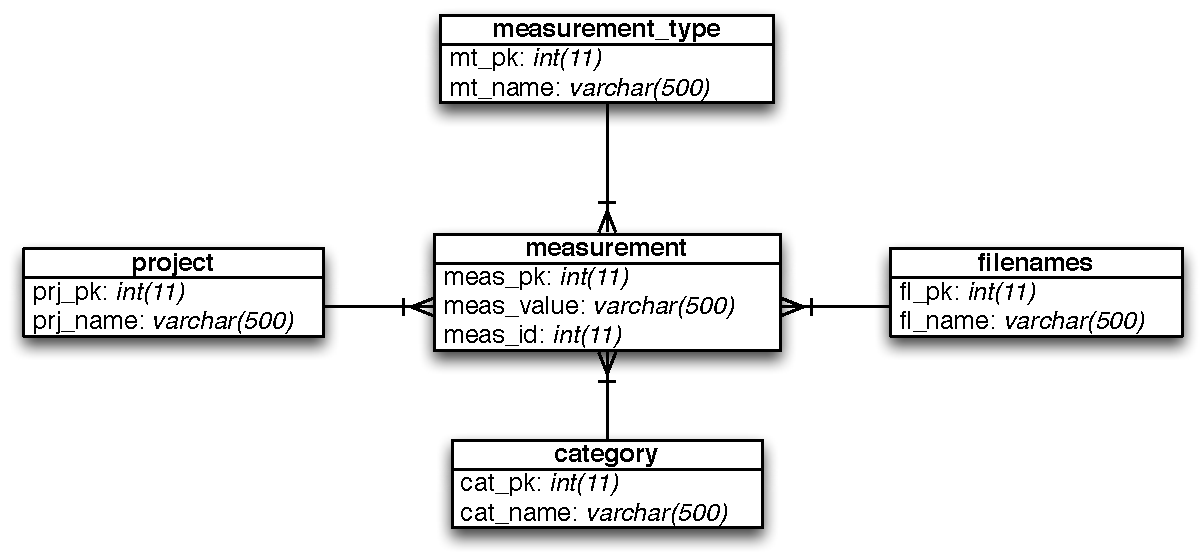
\includegraphics[scale=0.7]{database-schema}
\caption{The database schema}
\label{fig:database-schema}
\end{figure*}

\section{On the Use of Domain Specific Languages}
\label{sec:dsl}

The Java Platform exists more than a decade and provides a development environment for several application areas, such as web, grid computing, and traditional client-server applications. The official development environment of the Java platform is released by Oracle and is widely-known as the Java Standard Edition {\sc dsk}. The process of development and innovation in the Java ecosystem is built around a community, that writes proposals of features, known as {\sc jsr}s (Java Specification Requests), which are supported by prototype implementations.

In the literature, it is referred that {\sc dsl}s are used to reduce software development cost, by introducing domain efficiency \cite{MHS05}. This thesis focuses on practical research aspects as well as with the theoretical ones; thus the first problem that needs to be examined, is to measure the adoption of {\sc dsl}s in software projects. In addition, the average number of {\sc dsl}s usually used in a software project needs to be investigated.

The methodology was the following; A set of standard {\sc dsl} application libraries was identified, and the source was scanned for specific \textit{import} statements e.g. \textit{java.util.regex}, which indicated that the standard package that implements regular expressions was used, thus regular expressions were used. If a package is detected in the source code, then the project will be tagged that it uses one (1) {\sc dsl}. Consequently, if a project has {\sc dsl} count four (4), then it means that four (4) different application libraries were detected during the source code scan. Table \ref{tbl:dsl-list} lists the selected {\sc dsl}s application libraries. Note that all these libraries are included as part of the Java {\sc sdk}.

\begin{table}
\centering
\caption{List of selected DSL application libraries}
\label{tbl:dsl-list}
\begin{tabular}{l l}
 \hline
\textbf{DSL} & \textbf{Java Package}\\
\hline
Regular Expressions & \verb|java.util.regex|\\
XML & \verb|javax.xml|, \verb|org.w3c| and \verb|org.xml|\\
SQL & \verb|java.sql| and \verb|javax.sql|\\
XPath & \verb|java.xml.xpath|\\
XSLT & \verb|javax.xml.transform|\\
RTF & \verb|javax.swing.text.rtf|\\
HTML & \verb|javax.swing.text.html|\\
\hline
\end{tabular}
\end{table}

The initial goal of this experiment was simply to provide quantifiable results that are indicative regarding the usage of each {\sc dsl}, thus only files containing Java code were taken into account. Build files or other resources that may contain {\sc dsl}s were not included.

One final assumption was also made; if {\sc xpath} or {\sc xslt} were found in the source code, then the project would be marked that it also uses {\sc xml}, since those two languages are used for query and transformations on {\sc xml} {\sc dom} trees.

\begin{figure}
\centering
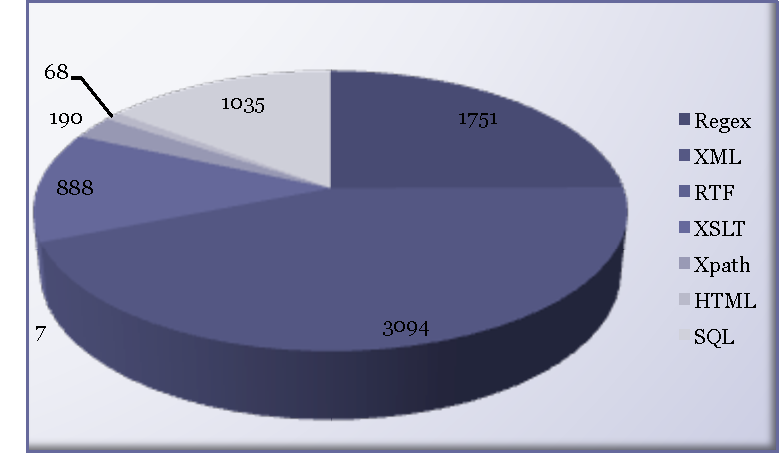
\includegraphics[scale=0.65]{dsl-usage}
\caption{DSL language usage in Java projects}
\label{fig:dsl-usage}
\end{figure}

\begin{table}
\centering
\caption{Popular DSL Usage Combinations}
\label{tbl:dsl-top-usage}
\begin{tabular}{l r}
 \hline
\textbf{DSLs} & \textbf{Count}\\
\hline
XML & 1,561\\
Regex & 909\\
SQL & 493\\
XML, XSLT & 475\\
Regex, XML, XSLT & 158\\
Regex, XML & 303\\
SQL, XML & 162\\
Regex, SQL & 116\\
Regex, SQL, XML, XSLT & 80\\
Regex, SQL, XML & 71\\
SQL, XML, XSLT & 54\\
XML, XPath & 50\\
XML, XPath, XSLT & 39\\
Regex, XML, XPath, XSLT & 38\\
HTML & 23\\
Regex, XML, XPath & 20\\
Regex, SQL, XML, XPath, XSLT & 18\\
SQL, XML, XPath, XSLT & 11\\
HTML, Regex, XML & 10\\
HTML, XML & 10\\
\hline
\end{tabular}
\end{table}

\section{Limitations}
\label{sec:limit}


\section{Related Work}
\label{sec:rel}

The Maven ecosystem has been previously analyzed by Raemaekers et al.~\cite{RDV13} to produce the {\it Maven dependency dataset}. Apart from basic information like individual methods, classes, packages and lines of code for every {\sc jar}, this dataset also includes a database with all the connections between the aforementioned elements. Our work differs from this research because it reports all bugs coming from the output of a static analysis tool, for each {\sc jar} contained in the Maven repository.

\cite{MKLGS14} \cite{KARA14}

\section{Conclusions}
\label{sec:conc}


\bibliographystyle{abbrv}
\bibliography{msr}

\end{document}
